\documentclass[10pt]{exam}

\usepackage{amssymb, amsmath, amsthm, mathrsfs, multicol, graphicx}
\usepackage{tikz}
\usepackage{array}

 \def\d{\displaystyle}
\def\?{\reflectbox{?}}
\def\b#1{\mathbf{#1}}
\def\f#1{\mathfrak #1}
\def\c#1{\mathcal #1}
\def\s#1{\mathscr #1}
\def\r#1{\mathrm{#1}}
\def\N{\mathbb N}
\def\Z{\mathbb Z}
\def\Q{\mathbb Q}
\def\R{\mathbb R}
\def\C{\mathbb C}
\def\F{\mathbb F}
\def\A{\mathbb A}
\def\X{\mathbb X}
\def\E{\mathbb E}
\def\O{\mathbb O}
\def\U{\mathcal U}
\def\pow{\mathcal P}
\def\inv{^{-1}}
\def\nrml{\triangleleft}
\def\st{:}
\def\~{\widetilde}
\def\rem{\mathcal R}
\def\sigalg{$\sigma$-algebra }
\def\Gal{\mbox{Gal}}
\def\iff{\leftrightarrow}
\def\Iff{\Leftrightarrow}
\def\land{\wedge}
\def\And{\bigwedge}
\def\AAnd{\d\bigwedge\mkern-18mu\bigwedge}
\def\Vee{\bigvee}
\def\VVee{\d\Vee\mkern-18mu\Vee}
\def\imp{\rightarrow}
\def\Imp{\Rightarrow}
\def\Fi{\Leftarrow}

%\def\={\equiv}
\def\var{\mbox{var}}
\def\mod{\mbox{Mod}}
\def\Th{\mbox{Th}}
\def\sat{\mbox{Sat}}
\def\con{\mbox{Con}}
\def\bmodels{=\joinrel\mathrel|}
\def\iffmodels{\bmodels\models}
\def\dbland{\bigwedge \!\!\bigwedge}
\def\dom{\mbox{dom}}
\def\rng{\mbox{range}}
\DeclareMathOperator{\wgt}{wgt}


\def\bar{\overline}


\newcommand{\vtx}[2]{node[fill,circle,inner sep=0pt, minimum size=4pt,label=#1:#2]{}}
\newcommand{\va}[1]{\vtx{above}{#1}}
\newcommand{\vb}[1]{\vtx{below}{#1}}
\newcommand{\vr}[1]{\vtx{right}{#1}}
\newcommand{\vl}[1]{\vtx{left}{#1}}
\renewcommand{\v}{\vtx{above}{}}

\def\circleA{(-.5,0) circle (1)}
\def\circleAlabel{(-1.5,.6) node[above]{$A$}}
\def\circleB{(.5,0) circle (1)}
\def\circleBlabel{(1.5,.6) node[above]{$B$}}
\def\circleC{(0,-1) circle (1)}
\def\circleClabel{(.5,-2) node[right]{$C$}}
\def\twosetbox{(-2,-1.4) rectangle (2,1.4)}
\def\threesetbox{(-2.5,-2.4) rectangle (2.5,1.4)}
\newcommand{\twoline}[2]{\begin{pmatrix}#1 \\ #2 \end{pmatrix}}


\def\circleA{(-.5,0) circle (1)}
\def\circleAlabel{(-1.5,.6) node[above]{$A$}}
\def\circleB{(.5,0) circle (1)}
\def\circleBlabel{(1.5,.6) node[above]{$B$}}
\def\circleC{(0,-1) circle (1)}
\def\circleClabel{(.5,-2) node[right]{$C$}}
\def\twosetbox{(-2,-1.5) rectangle (2,1.5)}
\def\threesetbox{(-2,-2.5) rectangle (2,1.5)}

%\pointname{pts}
\pointsinmargin
\marginpointname{pts}
\bonuspointname{pts}
\marginbonuspointname{pts}
\addpoints
\pagestyle{head}
%\printanswers

\firstpageheader{Math 228}{\bf Homework 6}{Due: Wednesday, October 11}


\begin{document}
\noindent \textbf{Instructions}: Same rules as usual -- turn in your work on separate sheets of paper.  You must justify all your answers for full credit.  Do not consult the internet.

\begin{questions}

\question[6] If you were to shade in a $n\times n$ square on graph paper, you could do it the boring way (with sides parallel to the edge of the paper) or the interesting way, as illustrated below:


\begin{center}
  \begin{tabular}{m{2cm}m{3cm}m{4cm}m{3cm}}
  \begin{tikzpicture}[scale=0.4]
    \draw (0,0) rectangle (1,1);
  \end{tikzpicture}
  &
  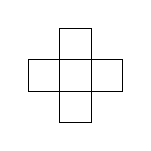
\begin{tikzpicture}[scale=0.4]
    \draw (-1,0) rectangle (2,1) (0,-1) rectangle (1,2);
  \end{tikzpicture}
  &
  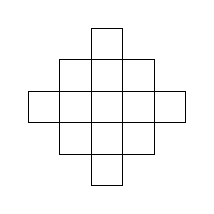
\begin{tikzpicture}[scale=0.4]
    \draw (-2,0) rectangle (3,1) (0,-2) rectangle (1,3) (-1,-1) rectangle (2,2);
  \end{tikzpicture}
  &
  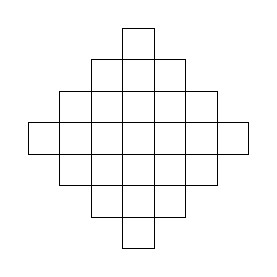
\begin{tikzpicture}[scale=0.4]
    \draw (-3,0) rectangle (4,1) (-2,-1) rectangle (3,2) (-1,-2) rectangle (2,3) (0,-3) rectangle (1,4);
  \end{tikzpicture}
\end{tabular}
\end{center}

The interesting thing here, is that a $3\times 3$ square now has area 13.  Our goal is the find a formula for the area of a $n \times n$ (diagonal) square.

\begin{parts}
  \part Write out the first few terms of the sequence of areas (assume $a_1 = 1$, $a_2 = 5$, etc).  Is the sequence arithmetic or geometric?  If not, is it the sequence of partial sums of an arithmetic or geometric sequence?  Explain why your answer is correct, referring to the diagonal squares.

  \begin{solution}
    The sequence is $1, 5, 13, 25, 41, 61, \ldots$.  This is not arithmetic
	  (since $5-1 = 4$ but $13-5 = 8$).  It is also not geometric (since $5/1 = 5$ but $13/5 = 2.6$).  To recognize whether the sequence is a sequence of partial sums, we look at the differences.  The sequence of differences is $4, 8, 12, 16, 20, \ldots$.  This {\em is} an arithmetic sequence.  So we see that
	  \[a_1 = 1\]
	  \[a_2 = 1+4\]
	  \[a_3 = 1+4+8\]
	  \[a_4 = 1+4+8+12\]
	  \[a_n = 1 + \sum_{k = 1}^n 4(k-1)\]
  \end{solution}

  \part Use your results from part (a) to find a closed formula for the sequence.  Show your work.  Note, while there are lots of ways to find a closed formula here, you should use partial sums specifically.
  \begin{solution}
    We have $a_n = 1 + 4 + 8 + \cdots + 4(n-1)$.  If we reverse these and add corresponding terms (not including the 1) we get
    \[2a_n = 2 + (4n) + (4n) + (4n) + \cdots + (4n)\]
    On the right hand side of the equation we have the sum of $n-1$ copies of $(4n)$ so we get
    \[2a_n = 2 + (n-1)(4n)\]
    or \[a_n = 2n^2 - 2n + 1\]
  \end{solution}
\end{parts}



\question[8] In their down time, ghost pirates enjoy stacking cannonballs in triangular based pyramids (aka, tetrahedrons), like those pictured here:

\centerline{

\begin{tikzpicture}
\draw (0,0) circle (10pt);
\draw[very thin, color=brown!15] (0,0) circle (10pt);
\shade[shading=axis,bottom color=black!70!brown, top color=black!15, shading angle=-40] (0,0) circle (10pt);
\end{tikzpicture}\qquad

\begin{tikzpicture}
\foreach \pos in {(-.32, .2), (.32,.2), (0,.55), (0,0)}{
\draw[very thin, color=brown!15] \pos circle (10pt);
\shade[shading=axis,bottom color=black!70!brown, top color=black!15, shading angle=-40] \pos circle (10pt);
}
\end{tikzpicture}
\qquad

\begin{tikzpicture}
\foreach \pos in {(-.64, .4), (.64,.4), (-.37, .75), (.37,.75), (0, 1.2), (-.32, .2), (.32,.2), (0,.6), (0,0)}{
\draw[very thin, color=brown!15] \pos circle (10pt);
\shade[shading=axis,bottom color=black!70!brown, top color=black!15, shading angle=-40] \pos circle (10pt);
}
\end{tikzpicture}
}

Note, these are solid tetrahedrons, so there will be some cannonballs obscured from view (the picture on the right has one cannonball in the back not shown in the picture, for example).


The pirates wonder how many cannonballs would be required to build a pyramid 15 layers high (thus breaking the world cannonball stacking record).  Can you help?  Find a closed formula for the number of cannonballs in the $n$th pyramid and use this to find the number of cannonballs in the 15th pyramid.

\begin{solution}
  To get the next larger pyramid, we add a triangle of cannonballs to the previous pyramid.  Thus to get $P_n$, we add $P_{n-1}$ to the $n$th triangular number:
  $P_3 = 4 + 6 = 10$, $P_4 = 10 + 10 = 20$, $P_5 = 20 + 15 = 35$.

  	To find the closed formula, look at the sequences of differences.  The first differences are $3, 6, 10, 15, \ldots$.  The second differences are $3, 4, 5, 6, \ldots$.  The third differences are $1,1,1,\ldots$.  Since third differences are constant, we know the closed formula for $P_n$ will be a degree 3 polynomial.  So $P_n = an^3 + b n^2 + cn + d$.  Note that $P_0 = 0$, so $d = 0$.  To solve for $a$, $b$, and $c$, we solve the system of equations:
  \begin{align*}
    1 & = a + b + c \\
    4 & = 8a+ 4b + 2c \\
    10 & = 27a + 9b + 3c
  \end{align*}
  Doing so gives $a = \frac{1}{6}$, $b = \frac{1}{2}$ and $c = \frac{1}{3}$ so
  \[P_n = \frac{1}{6}n^3 + \frac{1}{2} n^2 + \frac{1}{3} n\]

Finally:
  \[P_{15} = \frac{1}{6}15^3 + \frac{1}{2} 15^2 + \frac{1}{3} 15 = 680\]
\end{solution}




\question Let $a_n$ be the number of  $1 \times n$ tile designs can you make using $1 \times 1$ squares available in 4 colors and $1 \times 2$ dominoes available in 5 colors.
\begin{parts}
	\part[3] First, find a recurrence relation to describe the problem.  Explain why the recurrence relation is correct (your explanation should reference tile designs of squares and dominoes).
	\begin{solution}
		$a_n = 4a_{n-1} + 5a_{n-2}$.  Each path of length $n$ must either start with one of the 4 $1\times 1$ tiles, in each case there are then $a_{n-1}$ ways to finish the path, or start with one of the 5 $1\times 2$ tiles, in each case there are then $a_{n-2}$ ways to finish the path.
	\end{solution}

	\part[2] Write out the first 6 terms of the sequence $a_1, a_2, \ldots$.  Hint: since you have a recurrence relation, the only difficult part will be finding the first two terms, which are simple counting questions.
	\begin{solution}
		4, 21, 104, 521, 2604, 13021
	\end{solution}

	\part[3] Solve the recurrence relation.  That is, find a closed formula for $a_n$.
	\begin{solution}
		The characteristic equation is $x^2 - 4x - 5 = 0$ so the characteristic roots are $x = 5$ and $x = -1$.  Therefore the general solution is
		\[a_n = a 5^n + b (-1)^n\]
		We solve for $a$ and $b$ using the fact that $a_1 = 4$ and $a_2 = 21$.  We get $a = \frac{5}{6}$ and $b = \frac{1}{6}$.  Therefore the solution is
		\[a_n = \frac{5}{6} 5^n + \frac{1}{6}(-1)^n\]
	\end{solution}

\end{parts}


\question[8] Consider the sequences $2, 5, 12, 29, 70, 169, 408,\ldots$ (with $a_0 = 2$).
\begin{parts}
\part Describe the rate of growth of this sequence.
\begin{solution}
It does not seem to help to look at the difference between terms - in fact, the differences seem to be growing in the same manner as the original sequence.  However, looking at the ratio between terms gives us almost a common ratio of 2.  In other words, it appears that the sequence is growing exponentially.
\end{solution}


\part Find a recursive definition for the sequence.
\begin{solution}
We see that $5$ is a little more than twice the previous term, and 12 is a little more than twice 5.  In fact, it is exactly 2 more, which is the first term.  So perhaps $a_n = 2a_{n-1} + a_{n-2}$, and this seems to work moving forward.
\end{solution}

\part Find a closed formula for the sequence.  Don't be afraid to use the quadratic formula.

\begin{solution}
Use the characteristic root technique.  The characteristic equation is $x^2 - 2x - 1 = 0$.  Solving this (using the quadratic formula) gives $x = 1\pm\sqrt{2}$.  So we know that the closed formula for $a_n = a(1+\sqrt{2})^n + b(1-\sqrt{2})^n$.  Now let's find $a$ and $b$.  We have

\[2 = a + b\]
\[5 = a(1+\sqrt{2}) + b(1-\sqrt{2})\]
Use substitution: $a = 2-b$ so $5 = (2-b)(1+\sqrt 2) + b(1-\sqrt{2})$ which simplifies to $b = 1-\frac{3}{2 \sqrt{2}}$.  This gives $a = 1+\frac{3}{2\sqrt 2}$.  Therefore
\[a_n = (1+\frac{3}{2\sqrt 2})(1+\sqrt{2})^n + (1-\frac{3}{2 \sqrt{2}})(1-\sqrt{2})^n\]
\end{solution}

\part If you look at the sequence of differences between terms, and then the sequence of second differences, the sequence of third differences, and so on, will you ever get a constant sequence?  Explain how you know.
\begin{solution}
You will never get a constant sequence of differences.  If you did, this would mean that the original sequence would be some polynomial.  But we have an exponential closed formula, so no polynomial will fit.
\end{solution}
\end{parts}

\bonusquestion[4] Bonus: For the sequence in problem 1, find the closed formula in as many interesting ways as you can.  Each unique explanation gets 1 point.

\begin{solution}
  There are lots of interesting things you can do here.  From what we have done with sequences, you could notice that the second differences are constant, so you know that the closed formula will be quadratic.  You could then use polynomial fitting, or simply compare the sequence to $n^2$ to find the pattern.  More inventive solutions include:
  \begin{enumerate}
    \item Look along the diagonals.  The $n$th figure will have $n$ diagonals of $n$ squares, and $n-1$ diagonals of $n-1$ squares.  Thus all together, the number of squares is $n^2 + (n-1)^2$.
    \item If you count the number of squares in each row starting at the top, you will have $1, 3, 5, \ldots, 2n-3, 2n-1, 2n-3, \ldots, 3, 1$.  So we can think of the total number of squares as being the sum of the first $n$ odd numbers (counting up) plus the sum of the first $n-1$ odd numbers (counting down).  But the sum of the first $n$ odd numbers is $n^2$, so again we find the total number of squares to be $n^2 + (n-1)^2$.
    \item Enclose the figure in a larger square with dimensions $2n-1 \times 2n-1$.  Then look at what part of that square you don't want.  You have 4 triangles you must remove.  The $n$th figure requires removing a triangle with base $n-1$ on each corner, so we must remove $4T_{n-1}$, where $T_n = \frac{n(n+1)}{2}$ is the $n$th triangular number.  Thus the total number of squares in the figure is
    \[(2n-1)^2 - 4\frac{(n-1)n}{2}.\]
  \end{enumerate}
\end{solution}


\end{questions}
\end{document}
